\documentclass[a4paper,12pt]{report} %размер бумаги устанавливаем А4, шрифт 12пунктов


\usepackage[T2A]{fontenc}

\usepackage[utf8]{inputenc}%включаем свою кодировку: koi8-r или utf8 в UNIX, cp1251 в Windows

\usepackage[english,russian]{babel}%используем русский и английский языки с переносами

\usepackage[indentfirst,compact,topmarks,calcwidth,pagestyles]{titlesec}
\usepackage{titletoc}

\usepackage{amssymb,amsfonts,amsmath,mathtext,cite,enumerate,float} %подключаем нужные пакеты расширений

\usepackage{graphicx} %хотим вставлять в курсовой/диплом рисунки?
\graphicspath{{images/}}%путь к рисункам

\makeatletter
\renewcommand{\@biblabel}[1]{#1.} % Заменяем библиографию с квадратных скобок на точку:
\makeatother

\usepackage{geometry} % Меняем поля страницы
\geometry{left=1cm}% левое поле
\geometry{right=1.5cm}% правое поле
\geometry{top=1cm}% верхнее поле
\geometry{bottom=2cm}% нижнее поле

\renewcommand{\theenumi}{\arabic{enumi}}% Меняем везде перечисления на цифра.цифра
\renewcommand{\labelenumi}{\arabic{enumi}}% Меняем везде перечисления на цифра.цифра
\renewcommand{\theenumii}{.\arabic{enumii}}% Меняем везде перечисления на цифра.цифра
\renewcommand{\labelenumii}{\arabic{enumi}.\arabic{enumii}.}% Меняем везде перечисления на цифра.цифра
\renewcommand{\theenumiii}{.\arabic{enumiii}}% Меняем везде перечисления на цифра.цифра
\renewcommand{\labelenumiii}{\arabic{enumi}.\arabic{enumii}.\arabic{enumiii}.}% Меняем везде перечисления на цифра.цифра



\begin{document}
\begin{titlepage}
\newpage

\begin{center}
\vspace{7cm}
Московский Государственный Университет \\*
имени М.В. Ломоносова \\*
Факультет вычислительной математики и кибернетики \\*
Кафедра системного программирования \\
\end{center}

\vspace{16em}

\begin{center}
\Large Курсовая работа
\end{center}

\begin{center}
\Large{\textbf{Извлечение информации \linebreak из неструктурированных текстовых источников \linebreak с использованием имеющихся табличных данных}}
\end{center}

\vspace{10em}

\begin{flushright}
Выполнил: \\
Студент 327 группы \\
Бабичев Антон Витальевич \\
\vspace{1.5em}
Научный руководитель: \\
Недумов Ярослав Ростиславович \\
\end{flushright}

\vspace{\fill}

\begin{center}
Москва \\
2014
\end{center}

\end{titlepage}% это титульный лист
\tableofcontents % это оглавление, которое генерируется автоматически
\chapter*{Введение}
\addcontentsline{toc}{chapter}{Введение}

Анализ информации является важной задачей во многих отраслях человеческой деятельности, таких как наука, производство, экономика. Информации в наши дни очень много, и накапливается она усиленными темпами. Однако большинство информации имеет неудобную для интерпретации форму. В частности, текст может быть абсолютно неструктурирован и не подчинен каким-либо правилам. Работа с такими данными занимает большое количество времени, поэтому естественно желание упростить, ускорить и автоматизировать эту задачу. Далее эти данные используются для дальнейшего анализа.

Наибольшее количество информации сосредоточено в Интернете, и в основном она представлена в виде web-страниц. Данные об одном и том же объекте могут встречаться на разных сайтах, и информация, которую в себе несут эти данные, может друг друга дополнять. Использование единой структурированной базы знаний об объектах какого-либо типа очень полезно и упрощает анализ неструктурированных данных о них. Информация, полученная в результате анализа такого неструктурированного текста, несет пользу и помогает дополнить наши знания об определенном объекте. Например, мы можем дополнить базу знаний записью о новом объекте, если его параметры схожи по типу с таковыми у объектов в базе знаний. Либо мы можем дополнить запись об уже существующем в базе объекте новыми параметрами-характеристиками объекта. Также полезно уметь свзывать данные об одном и том же объекте с разных страниц в Интернете, чтобы, например, проверить имеющиеся знания в базе либо же дополнить ее.

В данной курсовой работе сконцентрировано внимание на извлечении информации из неструктурированного источника с использованием базы знаний% это введение
\chapter{Постановка задачи}

Целью данной работы является исследование и разработка методов извлечения информации из неструктурированного текстового источника. Для достижения данной цели были поставлены следующие задачи:

\begin{enumerate}
\item Исследовать существующие методы извлечения информации из текстовых источников
\item Разработать алгоритм извлечения информации из неструктурированных текстовых данных об объекте какого-либо типа с использованием доступной базы знаний об объектах того же типа
\item Создать прототип системы извлечения информации, подтверждающий работоспособность данного метода
\item Произвести оценку результатов разработанного метода 
\end{enumerate}
% это 1-я глава - Постановка задачи
\chapter{Обзор существующих решений}


\section{Методы, основанные на распозавании именованных сущностей}

Это группа методов, в основе которых лежат техники распознавания именованных сущностей. Именованная сущность - это группа слов в тексте, которая описывает реальный объект. Например, ``Apple Inc.'', ``John Broun'', ``information extraction'' и т.д. Поиск каких-либо именованных сущностей ведется в тексте с помощью паттерна. По способу нахождения паттерна методы делятся на подходы, основанные на правилах, и на статистические подходы.

Методы, основанные на правилах, (например, [1]) находят паттерн в тексте, редуцируя обобщенные правила. Например, из правила ``является числом'' получаются более специфичные правила ``является 4-значным числом'' или ``является дробным числом''. Для вычисления правил используются размеченная вручную обучающая база, поэтому для больших текстов данный подход неприменим.

Статистические подходы (например, система Nymble [2]) используют вариации EM-алгоритма для нахождения распределений токенов по сущностям. В частности, в Nymble использубтся скрытые Марковские модели. Поскольку предположение, что токены сущности распределены по нормальному закону во всем тексте может быть неприемлемо в случае неструктурированного источника, данный подход нам также неинтересен.

\section{Методы, основанные на NLP}

Методы (например, [3]) этой группы используют в вычислениях предположение о наличии структуры естественного языка в текстовом источнике, поэтому для нашей задачи не годятся.


\section{Методы, основанные на использовании базы знаний}

Данная группа методов представлена подходом, описанным Matthew Michelson и Craig A. Knoblock [4] и характеризуется использованием при анализе содержания текста некой базы знаний об объектах какого-либо типа. Анализируемый текст авторы подхода рассматривают просто как набор токенов без какой-либо структуры --- так называемый ``текстовый пост''. База знаний представлена записями об объектах в виде совокупности пар \{атрибут: значение\} и в рамках статьи называется ``множество элементарных исходов''. В своей статье авторы описывают рещение задачи разметки токенов поста заданным набором меток-атрибутов и особой метки ``junc'', символизирующей непринадлежность токена ни одному из атрибутов объекта.

Решается задача в несколько этапов: 
\begin{enumerate}
	\item Из множества элементарных исходов с помощью приблизительного сравнения выбирается подмножество записей.
	\item По посту и каждой отобранной записи строится вектор признаков
	\item Вектор признаков попадет на вход SVM-классификатору, обученному относить запись к одному из 2 классов: \textit{запись является схемой поста} и \textit{запись не является схемой поста}
	\item Лучший кандидат становится схемой поста
	\item По схеме поста и каждому токену поста строится вектор признаков
	\item Вектор признаков попадет на вход Multi-Class SVM-классификатору, обученному каждому токену поста ставить в соответствие метку-атрибут
	\item Для группы токенов одного атрибута проводится чистка --- отсеиваются токены с меткой ``junc''
	\item Остается размеченный пост - требуемый результат работы.
\end{enumerate}

Результат работы алгоритма меряется $F_1 \text{мерой}$ и составляет 0.7704.

Данный подход интересен тем, что решает задачу извлечения информации для полностью лишенного структуры источника. Также для обучения классификаторов не требуется размеченных вручную данных.% это 2-я глава - Обзор существующих решений
\chapter{Исследование и построение решения}

Для реализации решения был выбран подход, предложенный АФФТАРОМ, поскольку он создан для решения проблемы извлечения информации именно в неструктурированном тексте. Авторы подхода предлагают находить решение с помощью так называемого множества элементарных исходов. Каждый элемент этого множества представляет собой совокупность пар \{атрибут: значение\} и описывает ровно один объект из имеющейся базы знаний.

В рамках решения поставленной задачи необходимо решить следующие подзадачи:
\begin{enumerate}
	\item Поиск примерной схемы поста
	\item Извлечение информации
\end{enumerate}

Рассмотрим подробнее каждую из подзадач.


\section{Поиск примерной схемы поста}

Сперва необходимо выяснить структуру поста. Для этого пост сравнивается с элементами множества элементарных исходов (назовем его множеством кандидатов). Для каждого кандидата строится вектор признаков, который затем подается на вход классификатору, обученному относить вектор к одному из 2 классов: \textit{кандидат соответствует посту} и \textit{кандидат не соответствует посту}. Искомой схемой поста является кандидат, отнесенный к классу схем с наибольшей вероятностью.

Эта задача решается в 2 шага;
\begin{enumerate}
	\item Предобработка (построение подмножества кандидатов)
	\item Связывание (построение векторов и классификация)
\end{enumerate}

Рассмотрим подробнее каждый из шагов.


\subsection{Предобработка}

Каждый элемент вектора признаков представляет собой значение определенной меры, вычисленной для поста и конкретного атрибута кандидата либо кандидата в целом. Поскольку кандидат содержит в среднем около 20 атрибутов, а набор мер состоит из 6 мер, вычисление каждой из которых подразумевает сравнение строк, построение вектора признаков является недешевой операцией. В множестве кандидатов находится около десятка тысяч элементов, поэтому построение векторов признаков для каждого кандидата - достаточно длительная задача. Поэтому с помощью приблизительного сравнения выбирается подмножество кандидатов, для которого в дальнейшем и будет производиться классификация.

Для этого множество кандидатов кластеризуется по значениям нескольких конкретных атрибутов. В один кластер попадает группа кандидатов с одинаковыми значениями атрибутов, указанных при кластеризации. Один кластер может быть описан в виде правила, которому удовлетворяют все элементы этого кластера. Правило удобно представлять в виде конъюнкции пар \{атрибут: значение\}. Например, пусть множество кандидатов состоит из 4 элементов:

\begin{tabular}{l l l l l}
	\{имя: ”стол”\} & \{длина: 120\} & \{ширина: 80\} & \{материал: ”дерево”\} & [1]\\
	\{имя: ”стол”\} & \{длина: 120\} & \{ширина: 60\} & \{материал: ”стекло”\} & [2]\\
	\{имя: ”табурет”\} & \{длина: 70\} & \{ширина: 70\} & \{материал: ”дерево”\} & [3]\\
	\{имя: ”табурет”\} & \{длина: 60\} & \{ширина: 60\} & \{материал: ”сталь”\} & [4]\\
\end{tabular}
\linebreak
Тогда правилу \{имя: “стол”\}\{длина: 120\} соответствуют элементы 1 и 2, а правилу \{имя: “табурет”\}\{материал: “сталь”\} - 4 элемент. 

Обрабатывать и классифицировать в дальнейшем предстоит элементы одного выбранного кластера. Выбираемый кластер должен соответствовать 2 требованиям:
\begin{enumerate}
	\item Он должен состоять из как можно меньшего числа элементов (чтобы строить меньше векторов признаков)
	\item Он должен иметь достаточно элементов, чтобы содержать кандидатов, наиболее похожих на содержание поста - \textit{перспективных кандидатов}
\end{enumerate}

Для контроля требований над правилом вводятся 2 меры: 
\begin{itemize}
	\item $Reduction Ratio (RR) = 1 - \frac{C}{N}$, где $C$ --- мощность кластера, описываемого правилом, а $N$ --- мощность множества элементарных исходов
	\item $Pair Completeness (PC) = \frac{T_n}{S_n}$, где $T_n$ --- мощность множества перспективных кандидатов, содержащихся в кластере, описываемом правилом, а $S_n$ --- мощность множества перспективных кандидатов в множестве всех кандидатов.
\end{itemize}

Задача нахождения подмножества кандидатов сводится к нахождению правил, описывающих систему кластеров, содержащих всех перспективных кандидатов. Для этого используется sequentional covering algorythm, суть которого в следующем:\\

\noindent 
\textit{\textbf{перспективные кандидаты} = множество элементов, требующих покрытия\\
\textbf{система правил} = пустое множество\\
пока \textbf{перспективные кандидаты} не пусто, выполнить:\\
\-\hspace{1cm}	найти одно правило\\
\-\hspace{1cm}	убрать из \textbf{перспективные кандидаты} элементы, которые оно покрывает\\
\-\hspace{1cm}	добавить найденное правило к \textbf{система правил}\\
\textbf{результат} - \textbf{система правил}\\
} %textit

На каждом шаге ищется правило, максимизирующее $RR$ и имеющее $PC >= 0.5$. Для его поиска используется следующий алгоритм:\\

\noindent 
\textit{\textbf{атрибуты} = множество всех атрибутов\\
\textbf{кандидаты} = множество кандидатов для покрытия\\
\textbf{правило} = пустое множество\\
пока \textbf{атрибуты} не пусто, выполнить:\\
\-\hspace{1cm}	\textbf{часть правила} = \textbf{правило}\\
\-\hspace{1cm}	для каждой пары \{атрибут: значение\} из \textbf{атрибуты} выполнить:\\
\-\hspace{2cm}	добавить к \textbf{часть правила} пару \{атрибут: значение\}\\
\-\hspace{2cm}	если RR(\textbf{часть правила}) > RR(\textbf{правило}) и PC(\textbf{часть правила}) $>= 0.5$, то\\
\-\hspace{3cm}	\textbf{правило} = \textbf{часть правила}\\
\-\hspace{2cm}	удалить из \textbf{часть правила} добавленную ранее пару\\
\-\hspace{1cm}	если \textbf{правило} не изменилось, то\\
\-\hspace{2cm}	\textbf{результат} - \textbf{правило}\\
\-\hspace{1cm}	иначе\\
\-\hspace{2cm}	удалить атрибут, добавленный в \textbf{правило}, со всеми значениями из \textbf{атрибуты}\\
\textbf{результат} - \textbf{правило}\\
} %textit


\subsection{Связывание}

Для поста и каждого кандидата из подмножества, полученного в ходе предобработки, строится вектор признаков $V_{rl}$, имеющий следующую структуру:\\

\noindent
\textit{$V_{rl}(\text{пост}, \text{кандидат})$ = (\\
\-\hspace{1cm}	$RL\_scores(\text{пост}, \text{атр}_1)$\\
\-\hspace{1cm}	$RL\_scores(\text{пост}, \text{атр}_2)$\\
\-\hspace{1cm}	\ldots\\
\-\hspace{1cm}	$RL\_scores(\text{пост}, \text{атр}_1 \text{атр}_2 \ldots\text{атр}_n)$\\
} %textit

Вектор $RL\_scores(str_1, str_2)$ имеет следующую структуру:\\

\noindent
\textit{$RL\_scores(str_1, str_2)$ = (\\
\-\hspace{1cm}	$JaccardSim(str_1, str_2)$\\
\-\hspace{1cm}	$LevensteinDist(str_1, str_2)$\\
\-\hspace{1cm}	$JaroWinklerSim(str_1, str_2)$\\
\-\hspace{1cm}	$SmithWatermanSim(str_1, str_2)$\\
\-\hspace{1cm}	$Soundex(str_1, str_2)$\\
\-\hspace{1cm}	$PorterStemmer(str_1, str_2)$\\
} %textit

Для полученных векторов проводится процедура binary rescoring, которая заключается в приведении векторов действительных чисел к двоичным векторам. Правило приведения таково: компонента вектора становится 1, если ее значение максимально среди значений этой же компоненты всех остальных векторов, и 0, если иначе. Если несколько векторов обладают максимальным значением какой-либо компоненты, то у всех этих векторов компонента в процессе binary rescoring станет равной 1. Например, следующие вектора

\begin{tabular}{l l l l l l l}
	( & 0.21 & 0.0 & 0.5 & -0.2 & 3.0 & )\\
	( & 0.5 & 0.0 & 0.5 & -0.3 & 2.0 & )\\
	( & -0.12 & 0.3 & 0.3 & -0.7 & 3.0 & )\\
\end{tabular}
\linebreak
после binary rescoring выглядят так:

\begin{tabular}{l l l l l l l}
	( & 0 & 0 & 1 & 1 & 1 & )\\
	( & 1 & 0 & 1 & 0 & 0 & )\\
	( & 0 & 1 & 0 & 0 & 1 & )\\
\end{tabular}
\linebreak
Далее вектора подаются на вход классификатору SVM, обученному относить вектор к одному из 2 классов: \textit{кандидат соответствует посту} и \textit{кандидат не соответствует посту}. Среди всех кандидатов, отнесенных к классу \textit{кандидат соответствует посту} выбирается единственный, чье отнесение к данному классу сделано классификатором с большей вероятностью. Выбранный кандидат является схемой поста.


\section{Извлечение информации}

На этом шаге для найденной схемы и каждого токена поста строится вектор признаков $V_{ie}$, имеющий следующую структуру:\\

\noindent
\textit{$V_{ie}(\text{токен}, \text{схема})$ = (\\
\-\hspace{1cm}	$IE\_scores(\text{токен}, \text{атр}_1)$\\
\-\hspace{1cm}	$IE\_scores(\text{токен}, \text{атр}_2)$\\
\-\hspace{1cm}	\ldots\\
\-\hspace{1cm}	$IE\_scores(\text{токен}, \text{атр}_n)$\\
} %textit

Вектор $IE\_scores(str_1, str_2)$ имеет следующую структуру:\\

\noindent
\textit{$RL\_scores(str_1, str_2)$ = (\\
\-\hspace{1cm}	$LevensteinDist(str_1, str_2)$\\
\-\hspace{1cm}	$JaroWinklerSim(str_1, str_2)$\\
\-\hspace{1cm}	$SmithWatermanSim(str_1, str_2)$\\
\-\hspace{1cm}	$Soundex(str_1, str_2)$\\
\-\hspace{1cm}	$PorterStemmer(str_1, str_2)$\\
} %textit

Далее вектора подаются на вход классификатору Multi-Class SVM, обученному каждому токену поста ставить в соответствие метку того атрибута, к которому наиболее вероятно токен принадлежит. После этого для группы токенов, отнесенных к одному и тому же атрибуту, проводится процедура чистки, а именно изменения метки токена, который на самом деле не являются значением выбранного атрибута, на ``пустышку''. ``Пустышками'' в посте являются токены, которые не принадлежат значениям ни одного из атрибутов. Например, в объявлении о продаже товара это могут быть токены ``cheap'', ``for sale'', ``used'' и т. д. Суть чистки следующая:\\

\begin{enumerate}
	\item Из группы токенов формируется значение атрибута в посте (например, строка``tok1 tok2 … tokn'')
	\item Для полученной строки и значения соотнесенного атрибута из схемы поста вычисляется 2 меры: JaccardSim и JaroWinklerSim. Полученные значения считаются базовыми
	\item Затем по очереди из строки убирается по одному токену, и для полученной строки и значения атрибута заново вычисляются меры
	\item Если значения обоих мер возросли по сравнению с базовыми, то полученные значения сами становятся базовыми, а убранный токен становится кандидатом на удаление (замещая предыдущего кандидата, если он был)
	\item После проверки всех токенов кандидату на удаление ставится метка ``пустышка''
	\item Процесс повторяется, пока в при проверке токенов удается найти хотя бы одного кандидата на удаление
	\item Когда кандидатов на удаление больше нет, проверяются текущие значения мер. Если они меньше необходимых минимумов (для каждой меры свой), то всем токенам атрибута ставится метка ``пустышка''
\end{enumerate}

После очистки атрибутов остается пост, каждый токен которого помечен меткой-атрибутом либо меткой-``пустышкой'' - требуемый в задаче результат.
% это 3-я глава - Исследование и построение решения
\chapter{Описание практической части}


\section{Инструментарий}

\begin{itemize}
	\item В качестве языка реализации выбран язык программирования Java
	\item В качестве реализации классификаторов используется библиотека libsvm
	\item В качестве реализации мер над строками используется библиотека secondstring
	\item Для сбора данных для обучения и тестирования написан краулер на Python с использованием библиотеки scrapy
	\item В качестве реализации перевода данных для обучения из формата JSON во внутреннее представление используется библиотека json-simple
\end{itemize}


\section{Общая схема работы}

\begin{enumerate}
	\item Из JSON-файла с базой знаний загружаются записи для множества элементарных исходов
	\item Из входного файла считываются текстовые посты для анализа (по одному на каждой строке) Далее для каждого поста:
	\begin{enumerate}
		\item Предобработка множества элементарных исходов и получение подмножества кандидатов
		\item Связывание поста со схемой
		\item Классификация токенов поста в соответствии со схемой
		\item Чистка атрибутов поста
		\item Результат записывается в файл в виде ``токен метка'' 
	\end{enumerate}
\end{enumerate}


\section{Архитектура системы}

Работа программы начинается с класса \textit{Main}.

Класс \textit{DataStore} служит внутренним представлением базы знаний, с помощью метода \textit{init$\_$base} загружаются данные для обучения и множества элементарных исходов.

Класс \textit{BlockSchemeLearner} с помощью метода \textit{sequential$\_$covering} осуществляет предобработку множества элементарных исходов.

Класс \textit{PostExplorer} осуществляет связывание и извлечение нинформации. Метод \textit{results} производит чистку и запись результатов в выходной файл

На рисунке изображена упрощенная диаграмма классов системы\\
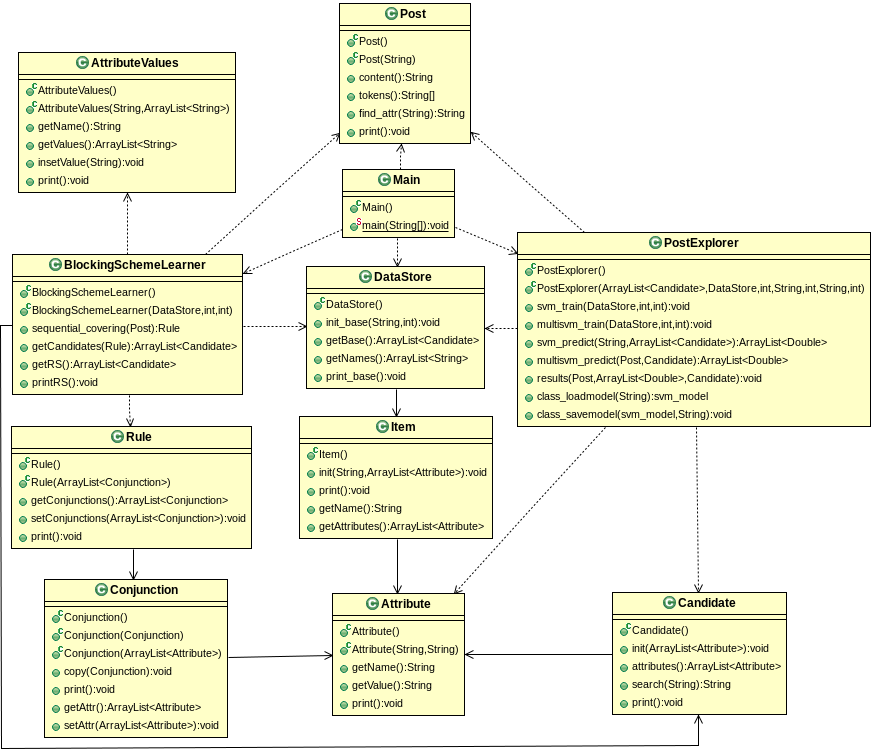
\includegraphics[width=\linewidth]{diagram.png}


\section{Анализ результатов}

Для тестирования работы алгоритма системе была поставлена задача разметки постов о ноутбуках в интернет-магазинах.

Для обучения SVM-классификатора использовались 8055 записей о ноутбуках с сайта amazon.com\footnote{www.amazon.com}. Для обучения Multi-Class SVM-классификатора по 8055 записям были искусственно созданы посты вида $\{\text{значение}\_\text{атрибута}_1 \ldots\text{значение}\_\text{атрибута}_n\}$. Для тестирования использовались 104 вручную размеченные записи о ноутбуках с сайта bestbuy.com\footnote{www.bestbuy.com}

Тестировалось качество разметки поста метками 6 атрибутов: цвет, диагональ экрана, RAM, объем внешней памяти, производитель, линейка

Для оценки качества использовалась $F_1 \text{мера} (\frac{2*Precision*Recall}{Precision + Recall}$). Значение меры вычислялось для каждого атрибута по-отдельности.\\

\begin{table}[H]
\caption{Результаты тестирования.}
\begin{center}
\begin{tabular}{|l|c|c|c|}
\hline
Атрибут & Precision & Recall & $F_1$\\
\hline
Цвет & 0.4462 & 0.7632 & 0.5631\\
Диагональ экрана & 0.9216 & 0.9592 & 0.94\\
RAM & 0.3789 & 0.72 & 0.4966\\
Память & 0.6094 & 0.7959 & 0.6903\\
Производитель & 0.8621 & 1.0 & 0.9259\\
Линейка & 0.2621 & 0.6585 & 0.375\\
\hline
Среднее & 0.58 & 0.8162 & 0.6652\\
\hline
\end{tabular}
\end{center}
\end{table}



В целом результат работы несколько хуже, чем таковой у авторов подхода. Этому может быть 2 причины.

1 причина заключается в неоднородности обучающей выборки Multi-Class SVM-классификатора и сильном разбросе значений атрибутов. Лучшее значение $F_1 \text{меры}$ достигнуто на атрибуте ``диагональ экрана'', этот атрибут есть почти у всех моделей и диапазон его значений довольно узок (около 10). В то время как атрибута ``линейка'' нет почти у половины записей в обучающей выборке, и диапазон значений очень широкий (его ширина сравнима с количеством записей).

2 причина заключается в процедуре чистки атрибутов и косвенно зависит от 1 причины. Из-за того, что в обучающей выборке недостаточно записей, содержащих, например, атрибут ``линейка'', то классификатор токен входного поста, относящийся к атрибуту ``линейка'' с большой вероятностью разметит другим атрибутом. В процессе чистки, таким образом, данный токен в лучшем случае станет ``пустышкой''. Поскольку пороговый минимум в конце чистки определяется исходя из обучающей выборки, а средняя длина значения атрибута ``линейка'' велика (более 15 символов), значения мер в чистке несколько больше, чем должно быть (так как ``мусорных'' токенов в посте обычно мало и они коротки). В результате страдает разметка токенов атрибутами, длина чьих значений очень мала (около 4 символов) - такие токены становятся ``пустышками''. Об этом свидетельствует низкая точность определения атрибута ``RAM''. % это 4-я глава - Описание практической части
\chapter*{Заключение}
\addcontentsline{toc}{chapter}{Заключение}

В рамках данной курсовой работы были получены следующие результаты:
\begin{enumerate}
	\item Исследованы существующие подходы к решению задачи извлечения информации из текстового источника.
	\item Разработан метод извлечения информации из неструктурированных текстовых данныых об объекте определенного типа с использованием доступной базы знаний по объектам того же типа.
	\item Создан прототип системы извлечения информации, подтверждающий работоспособность данного метода
	\item Произведена оценка качества результатов разработанного метода
\end{enumerate}
% это заключение
\chapter*{Список литературы}
\addcontentsline{toc}{chapter}{Список литературы}

\begin{enumerate}
	\item Mary Elaine Califf and Raymond J. Mooney. Relational learning of pattern-match rules for information extraction. In \textit{Proceedings of the 16th National Conference on Artificial Intelligence and the 11th Innovative Applications of Artificial Intelligence Conference}, pages 328-334, 1999.
	\item Daniel M. Bikel, Scott Miller, Richard Schwartz, Ralph Weischedel. Nymble: a High-Performance Learning Name-finder. In \textit{Proceeding ANLC 1997 Proceedings of the fifth conference on Applied natural language processing} pages 194-201, 1997.
	\item Frederik Hogenboom, Flavius Frasincar, Uzay Kaymak. An Overview of Approaches to Extract Information from Natural Language Corpora. \textit{DIR 2010 January 25, 2010, Nijmegen, the Netherlands}.
	\item Matthew Michelson and Craig A. Knoblock. Creating Relational Data from Unstructured and Ungrammatical Data Sources. In \textit{Journal of Artificial Intelligence Research 31 (2008)}, pages 543-590, 2008.
\end{enumerate}% это список литературы
\end{document}